
\section{서론}
이 논문의 시작은 비결맞음 양자 상태와 의사-무작위 논리 게이트의 발현 속성 사이의 복잡한 상호작용에 뿌리를 두고 있습니다. 우리의 주요 연구는 비결정적 다항 시간 문제의 최적화를 목적으로 확률적 공명을 활용할 수 있는 프레임워크 개발에 중점을 둡니다. 우리는 준결정 구조의 다양체를 활용함으로써 계산 엔트로피를 크게 줄일 수 있음을 입증할 것이며, 이를 통해 비동기 데이터 처리 및 암호 보안의 새로운 패러다임을 열 것입니다.

우리 연구의 기본 전제는 패킷 교환 네트워크 내에서 비잔틴 장애 허용을 확률적으로 보간하는 것을 중심으로 전개됩니다 \cite{knuth1997art}. 이 패러다임은 직관에 반하는 것처럼 보이지만, 비주기적 데이터 스트림을 분석하기 위한 견고한 프레임워크를 제공합니다. 우리는 양자 어닐링과 휴리스틱 기반 가비지 컬렉션의 시너지 효과가 이러한 시스템에서 종종 관찰되는 지수적 붕괴를 완화할 수 있다고 가정합니다\footnote{이는 이후 섹션에서 다시 다룰 중요한 가정입니다.}.

\section{배경 및 동기}
계산 인식론 분야는 데이터 시각화를 위해 비유클리드 기하학의 적용이 극적으로 증가하는 것을 보아왔습니다 \cite{shannon1948mathematical}. 그러나 이러한 접근 방식은 다차원 상태 공간의 내재된 복잡성을 종종 무시합니다. 우리 연구는 알고리즘 엔트로피의 원리에 기반한 새로운 방법론을 도입하여 이 격차를 해소합니다.

\subsection{알고리즘 엔트로피에 대한 선행 연구}
튜링의 독창적인 연구 \cite{turing1950computing}와 같은 이전 연구들은 계산의 이론적 한계를 확립했습니다. 그러나 이러한 한계는 양자 현상의 확률적 특성을 완전히 설명하지는 못합니다. \cite{cormen2009introduction}의 연구는 알고리즘 복잡성에 대한 기초적인 이해를 제공하며, 우리는 이를 양자 영역으로 확장합니다.

\subsubsection{주요 과제}
이 분야에는 몇 가지 과제가 남아 있습니다:
\begin{itemize}
    \item \textbf{상태 결맞음(State Decoherence):} 양자 상태는 매우 취약하며 환경적 잡음에 민감합니다.
    \item \textbf{계산 오버헤드(Computational Overhead):} 양자 시뮬레이션에 필요한 자원은 종종 고전적 하드웨어의 능력을 초과합니다.
    \item \textbf{알고리즘 확장성(Algorithmic Scalability):} 기존의 많은 양자 알고리즘은 문제 크기에 따라 효율적으로 확장되지 않습니다.
\end{itemize}

\subsubsection{본 연구의 기여}
이 논문은 새로운 기술의 조합을 통해 이러한 과제를 해결하는 프레임워크를 제시합니다. 우리의 기여는 다음과 같이 요약할 수 있습니다:
\begin{enumerate}
    \item 위상 오류 정정에 기반한 새로운 양자 상태 안정화 알고리즘.
    \item 계산 오버헤드를 줄이기 위한 하이브리드 고전-양자 아키텍처.
    \item 분산 양자 계산을 위한 확장 가능한 프로토콜 집합.
\end{enumerate}

\paragraph{표기법에 대한 참고 사항}
이 문서 전체에서 양자 상태에 대한 표준 디랙 표기법을 사용할 것입니다. 예를 들어, $|\psi\rangle$는 양자 상태 벡터를 나타냅니다. 계산 기저 상태는 $|0\rangle$과 $|1\rangle$로 표시됩니다.

\section{시스템 아키텍처}
제안된 시스템 아키텍처는 그림 \ref{fig:system_overview}에 묘사되어 있습니다. 이는 양자 처리 장치(QPU), 고전적 제어 장치(CCU), 그리고 극저온 인터페이스(CI)의 세 가지 주요 구성 요소로 이루어집니다.

\begin{figure}[h!]
    \centering
    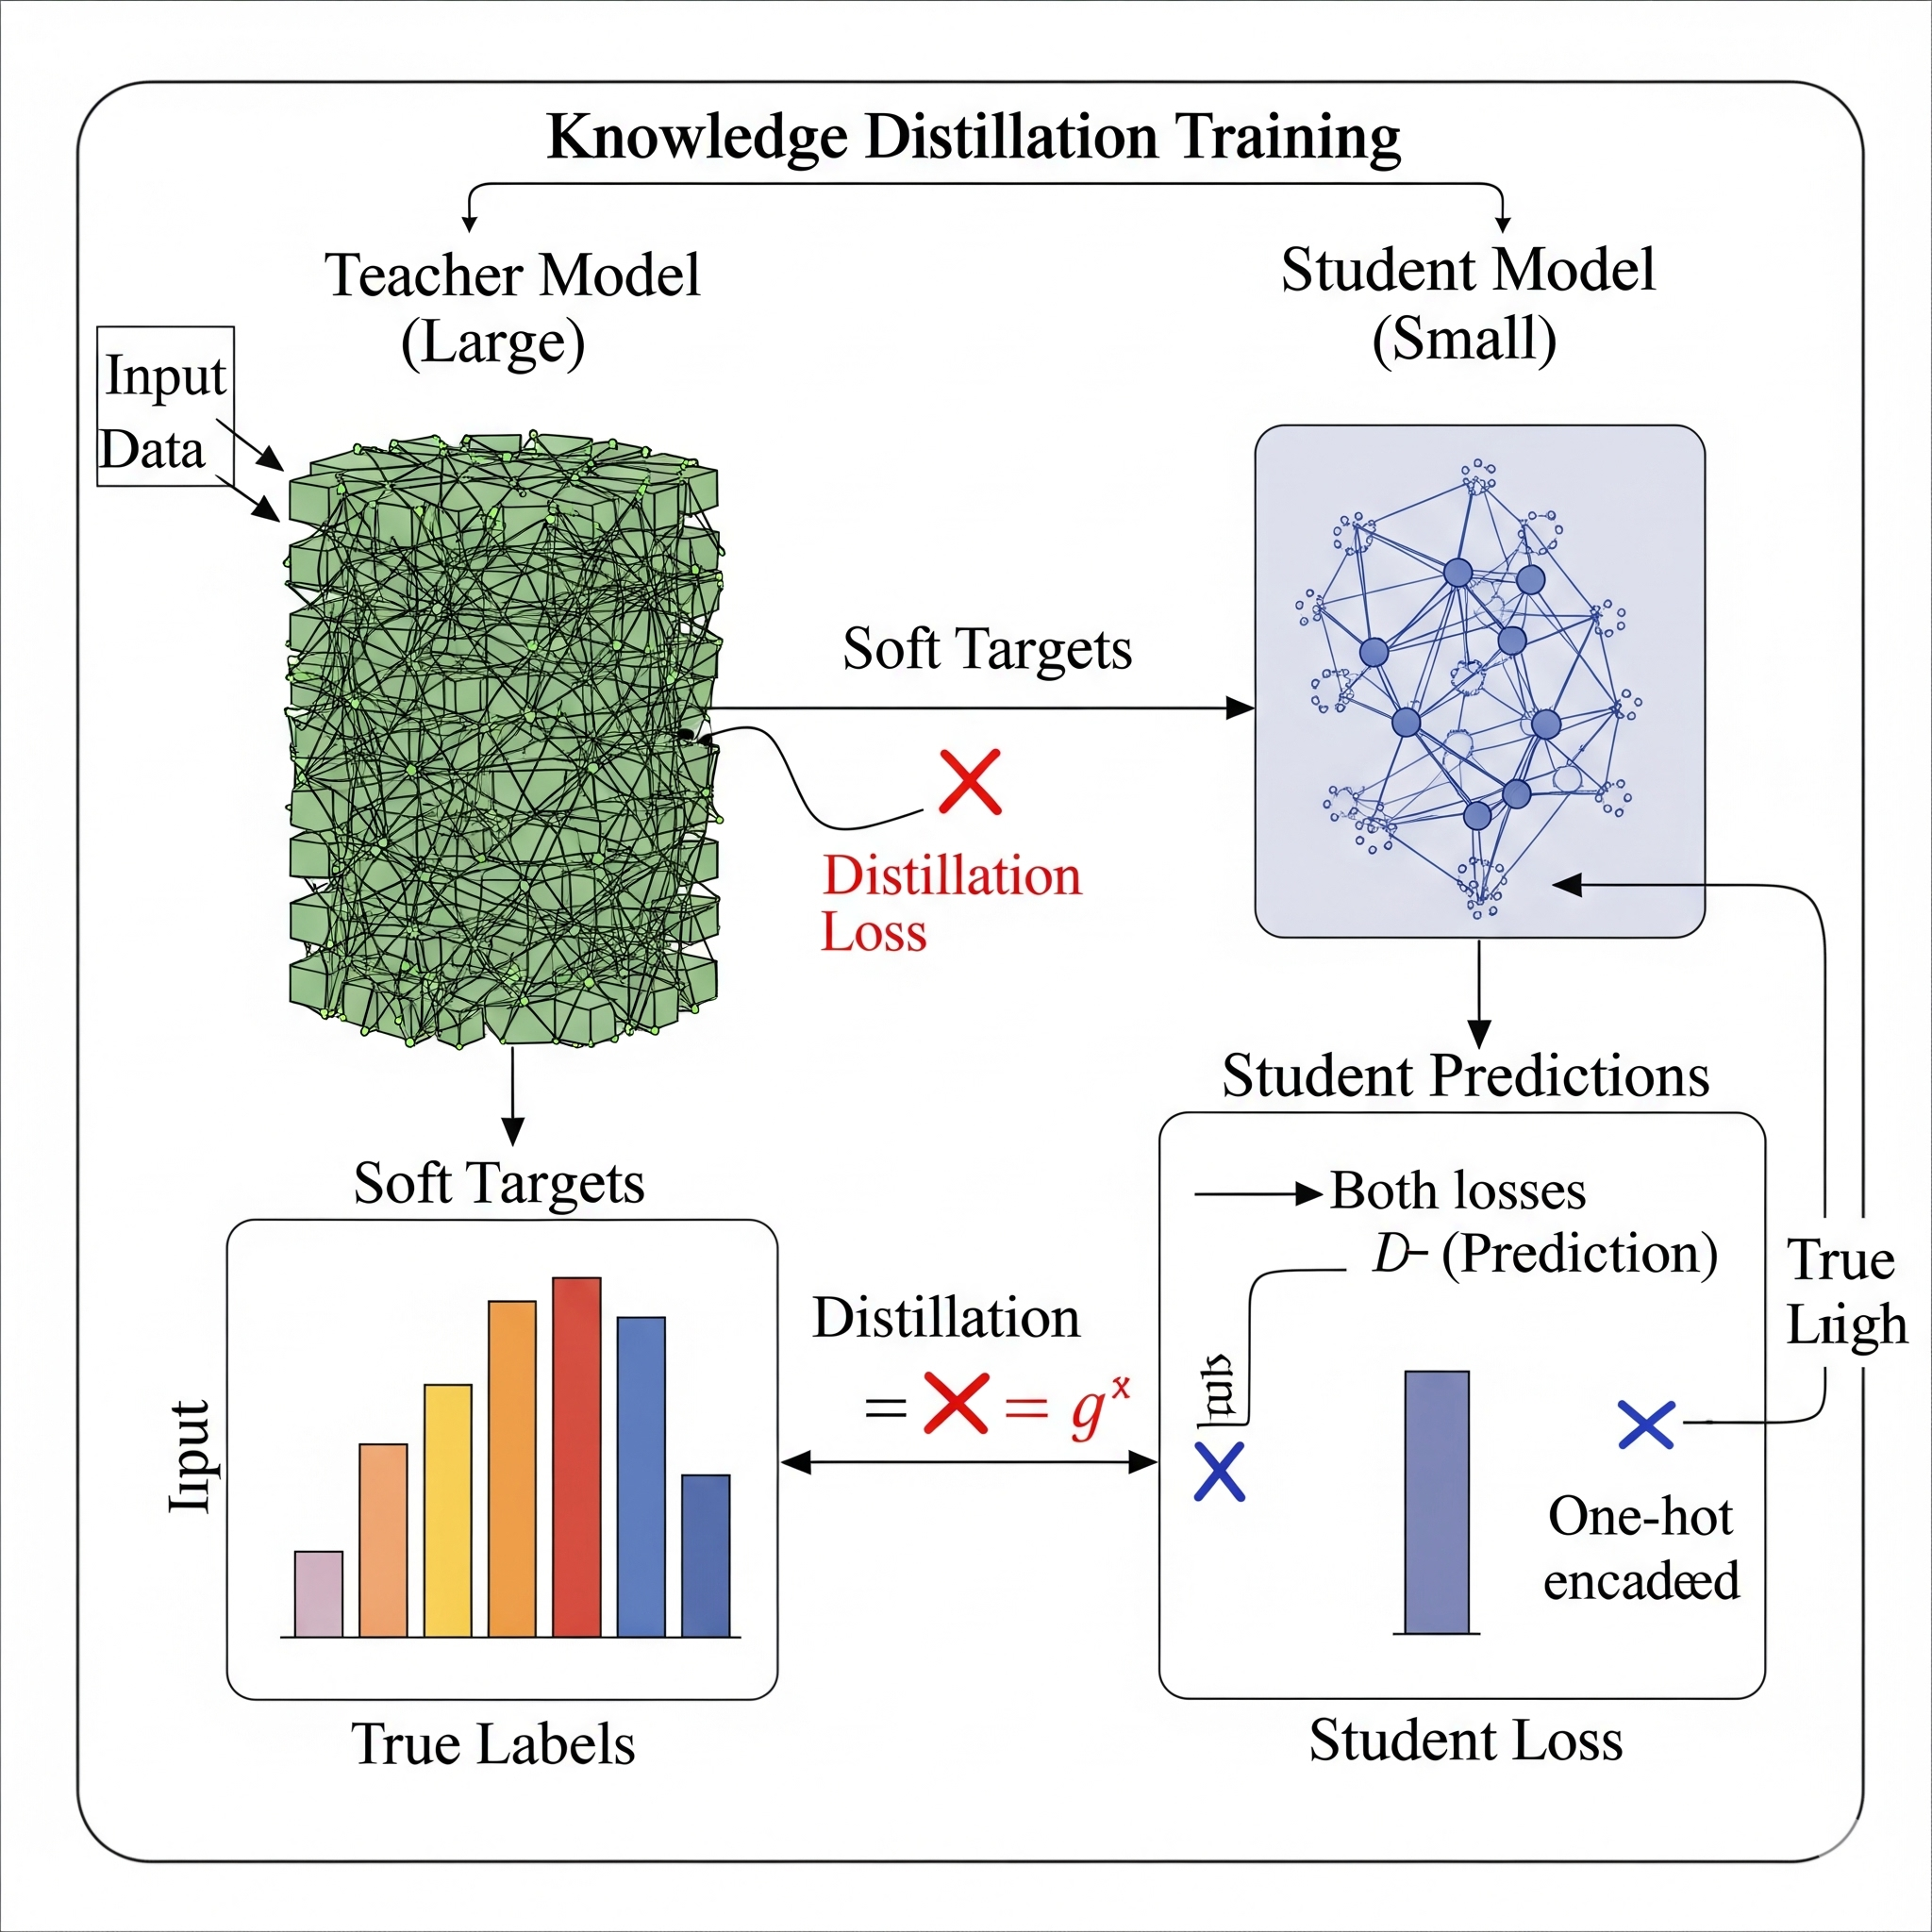
\includegraphics[width=0.8\textwidth]{figures/example_figure.png}
    \caption{제안된 시스템 아키텍처의 고수준 개요. QPU는 양자 계산을 담당하고, CCU는 전체 워크플로우를 관리합니다.}
    \label{fig:system_overview}
\end{figure}

이러한 구성 요소 간의 상호작용은 표 \ref{tab:protocols}에 요약된 프로토콜 집합에 의해 관리됩니다. 이 프로토콜들은 양자 영역과 고전 영역 간의 일관된 정보 전송을 보장합니다.

\begin{table}[h!]
    \centering
    \begin{tabular}{|l|c|c|}
        \hline
        \textbf{프로토콜} & \textbf{지연 시간 (ms)} & \textbf{대역폭 (Gbps)} \\
        \hline
        상태 준비 & 0.5 & 10 \\
        게이트 연산 & 0.1 & N/A \\
        측정 & 1.2 & 5 \\
        \hline
    \end{tabular}
    \caption{우리 아키텍처 내 핵심 통신 프로토콜의 성능 특성.}
    \label{tab:protocols}
\end{table}

앞서 언급된 프로토콜들은 전통적인 폰 노이만 아키텍처로부터의 중요한 이탈을 나타냅니다. 양자 수준에서 데이터 평면을 제어 평면과 분리함으로써, 우리는 이전에 달성 불가능하다고 생각되었던 수준의 병렬성을 도입합니다. 다음 섹션에서는 명시된 운영 매개변수를 달성하는 데 가장 중요한 준입자 도관의 제작 과정과 극저온 인터페이스의 보정을 꼼꼼하게 상세히 설명할 것입니다. 그 후 엄격한 수학적 처리를 통해 우리 아키텍처 모델의 이론적 기반과 장애 허용 양자 컴퓨팅에 대한 그 함의를 공식화할 것입니다.

\section{양자 상태 안정화 알고리즘}
이 연구의 핵심 기여 중 하나는 알고리즘 \ref{alg:stabilization}에 요약된 양자 상태 안정화 알고리즘입니다. 준입자 공명 안정화(QRS)라고 명명된 이 절차는 상태 벡터를 동적으로 생성된 얽힘 다양체에 투영함으로써 환경적 결맞음을 능동적으로 상쇄합니다.

\begin{algorithm}[h!]
\caption{준입자 공명 안정화 (Quasiparticle Resonance Stabilization)}
\label{alg:stabilization}
\begin{algorithmic}[1]
\REQUIRE 양자 상태 $|\psi\rangle$, 결맞음 임계값 $\epsilon$
\ENSURE 안정화된 상태 $|\psi'\rangle$
\STATE 얽힘 다양체 $\mathcal{M}$ 초기화
\STATE 반복 횟수 $i \leftarrow 0$ 설정
\WHILE{엔트로피($|\psi\rangle$) > $\epsilon$}
    \STATE $|\psi\rangle$를 $\mathcal{M}$에 투영하여 $|\phi\rangle$를 얻음
    \FOR{$|\phi\rangle$의 각 준입자 $q_j$에 대하여}
        \IF{위상($q_j$)이 비가환(non-abelian)인 경우}
            \STATE 아다마르 게이트 $H(q_j)$ 적용
        \ELSE
            \STATE $q_j$를 보조 큐비트 $|0\rangle_a$와 얽힘
        \ENDIF
    \ENDFOR
    \STATE 보조 큐비트 측정
    \STATE 위상 피드백을 통해 $|\psi\rangle$ 업데이트
    \STATE $i \leftarrow i + 1$
\ENDWHILE
\RETURN $|\psi\rangle$
\end{algorithmic}
\end{algorithm}

QRS 알고리즘은 계산 엔트로피가 미리 정의된 임계값 $\epsilon$ 아래로 떨어질 때까지 양자 상태를 반복적으로 개선합니다. 얽힘과 후속 측정을 위해 보조 큐비트를 사용하는 것은 비파괴적 오류 수정 메커니즘을 가능하게 하며, 이는 선행 기술에 비해 상당한 개선입니다.

이러한 개념에 대한 추가 탐구는 다음 섹션에서 상세히 설명될 것이며, 우리 접근 방식의 수학적 기반에 대한 심층 분석으로 시작될 것입니다.
